%----------------------------------------------------------------------------------------
% Fancy Article Template
% LaTeX Template
% Version 1.0
%
% Original author:
% Fiona Ding
%
% This template customizes the default article template for pretty notes.
%
% !TEX TS-program = pdflatex
% !TEX encoding = UTF-8 Unicode
%----------------------------------------------------------------------------------------


%----------------------------------------------------------------------------------------
%	PACKAGES AND OTHER DOCUMENT CONFIGURATIONS
%----------------------------------------------------------------------------------------     

\documentclass[11pt]{scrartcl} % use larger type; default would be 10pt; use Koma article

\usepackage[utf8]{inputenc} % set input encoding (not needed with XeLaTeX)
\usepackage[english]{babel} % English language

% --- PAGE DIMENSIONS ---
\usepackage{geometry} % to change the page dimensions
\geometry{letterpaper} % or letterpaper (US) or a5paper or....
% \geometry{margin=2in} % for example, change the margins to 2 inches all round
% \geometry{landscape} % set up the page for landscape
%   read geometry.pdf for detailed page layout information

\usepackage{graphicx} % support the \includegraphics command and options

\usepackage[parfill]{parskip} % Activate to begin paragraphs with an empty line rather than an indent

% --- FONT CUSTOMIZATIONS ---
\usepackage[T1]{fontenc}
\usepackage[osf]{mathpazo} % Palatino as the main font
\linespread{1.05}\selectfont % Palatino needs some extra spacing, here 5% extra
\usepackage[scaled=.88]{beramono} % Bera-Monospace
\usepackage[scaled=.86]{berasans} % Bera Sans-Serif

\usepackage[dvipsnames]{xcolor}  % Allows the definition of hex colors
\definecolor{titleblue}{rgb}{0.16,0.24,0.64} % Custom color for the title on the title page
\definecolor{linkcolor}{rgb}{0,0,0.42} % Custom color for links - dark blue at the moment

\addtokomafont{title}{\Huge\color{titleblue}} % Titles in custom blue color
\addtokomafont{author}{\color{darkgray}} % Author in dark gray
\addtokomafont{date}{\bfseries\color{gray}} % Date in gray
\addtokomafont{pagehead}{\normalfont\sffamily\color{gray}} % Header text in gray and sans serif
\addtokomafont{caption}{\footnotesize\itshape} % Small italic font size for captions
\addtokomafont{captionlabel}{\upshape\bfseries} % Bold for caption labels
\addtokomafont{descriptionlabel}{\rmfamily}
\setcapwidth[r]{10cm} % Right align caption text
%\setkomafont{footnote}{\sffamily} % Footnotes in sans serif

% --- PACKAGES ---
\usepackage{booktabs} % for much better looking tables
\usepackage{array} % for better arrays (eg matrices) in maths
\usepackage{paralist} % very flexible & customisable lists (eg. enumerate/itemize, etc.)
\usepackage{verbatim} % adds environment for commenting out blocks of text & for better verbatim
\usepackage{subfig} % make it possible to include more than one captioned figure/table in a single float
\usepackage{amsmath} % math!
%\usepackage{minted} % code!
\usepackage[
    urlcolor=linkcolor, % Color of URLs
    citecolor=linkcolor, % Color of citations
    linkcolor=linkcolor % Color of links to other pages/figures
]{hyperref}	% hyperlinks

% --- HEADERS & FOOTERS ---
\usepackage{fancyhdr} % This should be set AFTER setting up the page geometry
\pagestyle{fancy} % options: empty , plain , fancy
\renewcommand{\headrulewidth}{0pt} % customise the layout...
\lhead{}\chead{}\rhead{}
\lfoot{}\cfoot{\thepage}\rfoot{}

% --- TITLE APPEARANCE ---
\DeclareFixedFont{\textaut}{T1}{phv}{bx}{n}{0.8cm} % Font for author name: Helvetica 0.8 cm
\DeclareFixedFont{\textdt}{T1}{phv}{bx}{n}{0.6cm} % Font for author name: Helvetica 0.8 cm

% --- SECTION TITLE APPEARANCE ---
\usepackage{sectsty}
\allsectionsfont{\sffamily\bfseries\scshape} % sffamily: , bf: bold, scshape: small caps

% --- TABLE OF CONTENTS APPEARANCE ---
\usepackage[nottoc,notlof,notlot]{tocbibind} % Put the bibliography in the ToC
\usepackage[titles,subfigure]{tocloft} % Alter the style of the Table of Contents
\renewcommand{\cftsecfont}{\rmfamily\mdseries\upshape}
\renewcommand{\cftsecpagefont}{\rmfamily\mdseries\upshape} % No bold!


%----------------------------------------------------------------------------------------
%	TITLE PAGE
%----------------------------------------------------------------------------------------

\title{\fontsize{40pt}{40pt} \selectfont{CS-7280: Network Science}}
\author{\textaut{Fiona Ding}}
\date{\textdt{OMSCS Summer 2022}}

\begin{document}
\maketitle

%-----------------------------------------
% Table of Contents

\tableofcontents
\newpage

%----------------------------------------------------------------------------------------
%	DOCUMENT CONTENTS
%----------------------------------------------------------------------------------------

%-----------------------------------------
\section{Lesson 1: What is network science?}

Objectives:
\begin{itemize}
	\item Define "network science"
	\item Underestand its history and connections with other disciplines
	\item Applications of network science
\end{itemize}

Reading:
\begin{itemize}
	\item Chapter-1 from A-L. Barabási, \href{http://networksciencebook.com/}{Network Science}.
	\item Recommended papers:
	\begin{itemize}
		\item Networks in Epidemiology: \href{https://www.aaai.org/ojs/index.php/aimagazine/article/view/2283}{An Integrated Modeling Environment to Study the Co-evolution of Networks, Individual Behavior and Epidemics} by Chris Barrett et al.
		\item Networks in Biology: \href{http://www.plantcell.org/content/19/11/3327.short}{Network Inference, Analysis, and Modeling in Systems Biology} by Reka Albert
		\item Networks in Neuroscience: \href{http://www.nature.com/nrn/journal/v10/n3/full/nrn2575.html}{Complex brain networks: graph theoretical analysis of structural and functional systems} by Ed Bullmore and Olaf Sporns
		\item Networks in Social Science: \href{http://citeseerx.ist.psu.edu/viewdoc/download?doi=10.1.1.226.935&rep=rep1&type=pdf}{Network Analysis in the Social Sciences} by Stephen Borgatti et al.
		\item Networks in Economics: \href{https://www.sg.ethz.ch/publications/2009/schweitzer2009economic-networks-the/}{Economic Networks: The New Challenges} by Frank Schweitzer et al.
		\item Networks in Ecology: \href{https://www.sciencedirect.com/science/article/abs/pii/S1439179107000576?via\%3Dihub}{Networks in Ecology} by Jordi Bascompte
		\item Networks and the Internet: \href{http://www.ee.ucl.ac.uk/~mrio/papers/hamedjrnl_camera.pdf}{Network Topologies: Inference, Modelling and Generation} by Hamed Haddadi et al.
	\end{itemize}
\end{itemize}

\subsection{Lecture Notes}

% L1: Module 1
\subsubsection{Definition of network science}
\textbf{Definition:} The study of complex systems focusing on their architecture, i.e., on the network, or graph, that shows how the system components are interconnected.

% L1: Module 2-3
\subsubsection{Complex Systems}
Fundamental properties of the complex systems that network science is interested in:
\begin{itemize}
	\item Many and heterogeneous components
	\item Components that interact with each other through a non-trivial network (not connected randomly)
	\item Non-linear interactions between components
\end{itemize}

In contrast to complex networks:
\begin{itemize}
	\item \textbf{Regular networks} have the same interconnection pattern for all nodes; regular networks have been studied extensively by mathematicians.
	\item \textbf{Random networks} are networks where the connections between nodes are determined randomly.
\end{itemize}

Most networks in practice are not regular or random, they have interaction patterns that are highly variable.

% L1: Module 4
\subsubsection{Complex Systems and Their Network Representation}
Note that mapping an actual complex system to a graph representation is only a model. Some information about the system is lost in the model. Thus, it's always important to ask whether the network representation of a given system has enough detail to answer the questions you are interested in about the system.

% L1: Module 5
\subsubsection{Premise of Network Science}
The network architecture of a system provides valuable information about the system's function, capabilities, resilience, evolution, etc. We don't need to know all the details about the system and its components to draw conclusions about the system.

% L1: Module 6
\subsubsection{Examples of Network Science}
\begin{itemize}
	\item \textbf{a} -
	\item \textbf{b} -
\end{itemize}

% L1: Module 7
\subsubsection{Network Centrality}
The centrality of a node/edge is a measure of the "importance". There are different metrics that can be used to measure the centrality, eg:
\begin{itemize}
	\item number of other nodes that 
- causes largest disruption if removed
-
\end{itemize}

%%%%% TO BE CONTINUED %%%%%%

%-----------------------------------------
\subsection{Book: Chapter 1}


%%%%% TO BE CONTINUED %%%%%%

%-----------------------------------------
% LESSON 2
%-----------------------------------------
\section{Lesson 2: Graph Theory}

Objectives:
\begin{itemize}
	\item Review relevant concepts from graph theory and linear algebra
	\item Review basic graph algorithms 
	\item Explain how these concepts, math, algorithms relate to real-world networks
\end{itemize}

Reading:
\begin{itemize}
	\item Chapter-2 from A-L. Barabási, Network Science(Links to external site), 2015.
	\item Chapter-2 from D. Easley and J. Kleinberg, Networks, Crowds and Markets
	\item (Recommended) Fibonacci Heap. Wikipedia. \url{https://en.wikipedia.org/wiki/Fibonacci\_heap}
	\item (Recommended) Kosaraju's Algorithm. Wikipedia. \url{https://en.wikipedia.org/wiki/Kosaraju\%27s\_algorithm}
\end{itemize}

%-----------------------------------------
% LESSON 2: LECTURES
\subsection{Lecture Notes}

% L2: Module 1
\subsubsection{Undirected Graphs}
\textbf{Graph or Network:} collection of dyadic relations between a set of nodes (aka vertices). Relations are called edges or links. Represented by $G(V,E)$, where 

\textbf{Undirected Graph} \\
Graphs are often represented by an Adjacency Matrix or an Adjacency List. An adjacency matrix only needs a single memory access to check if an edge exists, but requires $n^2$ space; an adjacency list requires $n + 2*m$ where $n$ is the number of nodes and $m$ is the number of edges. For sparse graphs, where the number of edges is closer to $n$ than the max of $n-choose-2$, the size of an adjacency matrix vs list can differ by a lot. 


\subsubsection{Walks, Paths, Cycles}
A \emph{walk} can visit a node more than once.

A \emph{path} is a walk where the intermediate nodes are distinct.

A \emph{cycle} is a path that starts and ends on the same node.

The number of walks between two nodes of length $k$ is given by $A^k$, where A is the adjacency matrix.

\subsubsection{Connected Components}
An undirected graph is \textbf{connected} if there exists a path between any two nodes. Many real-world networks are not connected, but consist of multiple \textbf{connected components}. BFS can be used to obtain all the nodes in a connected component.

\subsubsection{Regular Networks}
\textbf{Trees} are connected graphs with no cycles.

A \textbf{k-regular graph} is a network where every vertex has the same degree k.

A \textbf{complete graph} , or a \textbf{clique}, is a special case of a k-regular network where every vertex is connected to every other vertex ($k=n-1$).

\subsubsection{Directed Graphs}
Each edge in directed graphs has a starting node and an ending node, ie the edge has a direction. Thus, the adjacency matrix may no longer be symmetric.

The definition of node degree for directed graphs now needs to be split into \textbf{in-degree} and \textbf{out-degree}.

\subsubsection{Weighted Graphs}
When edges can have different strengths, we can represent the strenth of the edge with a weight. For undirected graphs, the strength of a node is the sum of weights of all edges adjacent to the node. For directed graphs, we can define both an \textbf{in-strength}, the weight of all incoming edges, and an  \textbf{out-strength}, the weight of all outgoing edges.

 \textbf{Signed graphs} can have negative edge weights, which represent competitive interactions.

\subsubsection{Strongly Connected Components}
In directed graphs, the notion of \emph{connectedness} is different, since there may exist a path from node $s$ to node $t$ but not vice versa. 

A directed graph is \textbf{strongly connected} if there is a path between all pairs of vertices. A \textbf{strongly connected component} of a directed graph is a maximal strongly connected subgraph. 

\paragraph{How to determine if a directed graph is strongly connected?} 
The graph is strongly connected iff any node $s$ can reach every other node AND any other node can reach $s$. 
\begin{enumerate}
	\item Pick any node $s$.
	\item Run BFS from $s$ on the original graph, $G$ and see if the traversal reaches all nodes in $G$. This checks that $s$ can reach all nodes in the graph.
	\item Run BFS from $s$ on the reverse graph, $G'$, with all edges in the opposite direction of $G$, and see if the traversal reaches all nodes in $G'$. This checks that all other nodes have a path to $s$.
\end{enumerate}

\textbf{Note}: see Tarjan's algorithm and Kosaraju's algorithm to compute the set of strongly connected components in a directed graph.

\subsubsection{Directed Acyclic Graphs (DAG)}
A \textbf{DAG} is a directed graph that does not contain any cycles. They are common because they represent generalized hierarchies and dependency networks.

A graph has a \textbf{topological ordering} if we can run its nodes such that every edge points from a node of lower rank to a node of higher rank. 

Properties of DAGs:
\begin{enumerate}
	\item If a directed network has a topological ordering it must be a DAG.
	\item A DAG must have at least one source node, ie a node that does not contain any incoming edges.
	\item If a graph is a DAG it must have a topological ordering.
\end{enumerate}

The first and third properties can also be stated: a directed graph has a topological ordering if and only if it is a DAG.

\textbf{How to show the above properties:}
\paragraph{Topological ordering $\implies$ DAG} If the graph had a cycle, there would be an edge from a higher-rank node to a lower-rank node, which violates the topological order property.

\paragraph{At least one source node} Start from any node and start moving backwards. Since there are no cycles and the graph has a finite number of nodes, we must eventually reach a source node.

\paragraph{DAG $\implies$ Topological ordering} Start from a source node. Remove the node from the graph and decrement the in-degree of all nodes it pointed to. The graph is still a DAG. Choose a new source node and repeat until all nodes are removed.

\subsubsection{Dijkstra's Algorithm}
The shortest path(s) between a pair of nodes is often useful to know, since they represent the most effiecient way to move within a network. 

In unweighted networks, the shortest path can be found in linear time using BFS. If the network is weighted, Dijkstra's algorithm can be used to determine the shortest path.

\subsubsection{Random Walks}

\subsubsection{Min-Cut Problem}
A \textbf{$cut(s, t)$} is a set of edges in a graph such that if those edges were removed it would disrupt all paths between $s$ and $t$.

The \textbf{minimum cut} is the cut with the minimum sum of edge weights.

\subsubsection{Max-Flow Problem}
The flow from a source to a target node

\subsubsection{Bipartite Graphs}
A \textbf{bipartite graph} is a graph where the set of nodes can be partitioned into two subsets such that every edge connects a node from one subset to the other. No vertices within each subset are connected to each other.

\textbf{Theorem}: A graph is bipartite if and only if it does not include any odd-length cycles.

Bipartite graphs can be used for recommendation systems: eg given a bipartite graph mapping users to the items they bought. 
\begin{itemize}
	\item To find users with similar preferecnces, compute the \textbf{one-mode projection} of the bipartite graph onto the set of users. The projection contains only the user nodes, and an edge between two users if they have purchased at least one common item. 
	\item To find items that are often purchased together, compute the \textbf{one-mode projection} onto the set of items. Two items are connected with a weighted edge representing the number of users that purchased both items.
\end{itemize}

The \textbf{one-mode projections} can be computed using the adjacency matrix of the bipartite graph, $A$. 
\begin{itemize}
	\item The \textbf{co-citation metric}, $C_{i,j}$, between two nodes $i$ and $j$, is the number of nodes that have outgoing edges to both $i$ and $j$, ie, if $i$ and $j$ are items, $C_{i,j}$ is the number of users who purchased both $i$ and $j$. It can be computed: $C=A^T A$.
	\item The \textbf{bibliographic coupling metric}, $B_{i,j}$, between two nodes $i$ and $j$, is the number of nodes that receive incoming edges from both $i$ and $j$, ie, if $i$ and $j$ are users, $B_{i,j}$ is the number of items purchased by both $i$ and $j$. It can be computed: $B=A A^T$
\end{itemize}



%-----------------------------------------
% LESSON 2: Reading
\subsection{Reading Notes}

%-----------------------------------------
% LESSON 3
%-----------------------------------------
\section{Lesson 3: Degree Distribution and the "Friendship Paradox"}

Objectives:
\begin{itemize}
	\item Measure and interpret the degree distribution of a network
	\item Understand the “friendship paradox” to illustrate the importance of the degree distribution 
	\item Learn the G(n,p) model as the most basic type of random graph
	\item Degree correlations and assortative networks
\end{itemize}

Reading:
\begin{itemize}
	\item Chapter 3 from A-L. Barabási, \href{http://networksciencebook.com/}{Network Science}.
	\item Chapter 7, Sections 7.1, 7.2, 7.3, 7.5 from A-L. Barabási, \href{http://networksciencebook.com/}{Network Science}.
	\item (Recommended) \href{http://www.ploscompbiol.org/article/info\%3Adoi\%2F10.1371\%2Fjournal.pcbi.1001109#s2}{Simulated Epidemics in an Empirical Spatiotemporal Network of 50,185 Sexual Contacts}
\end{itemize}

%-----------------------------------------
% LESSON 3: LECTURES
\subsection{Lecture Notes}

% L3: Degree Distribution
\subsubsection{Degree Distribution}
The degree distribution shows the fraction of nodes with degree k.
	\begin{center}
		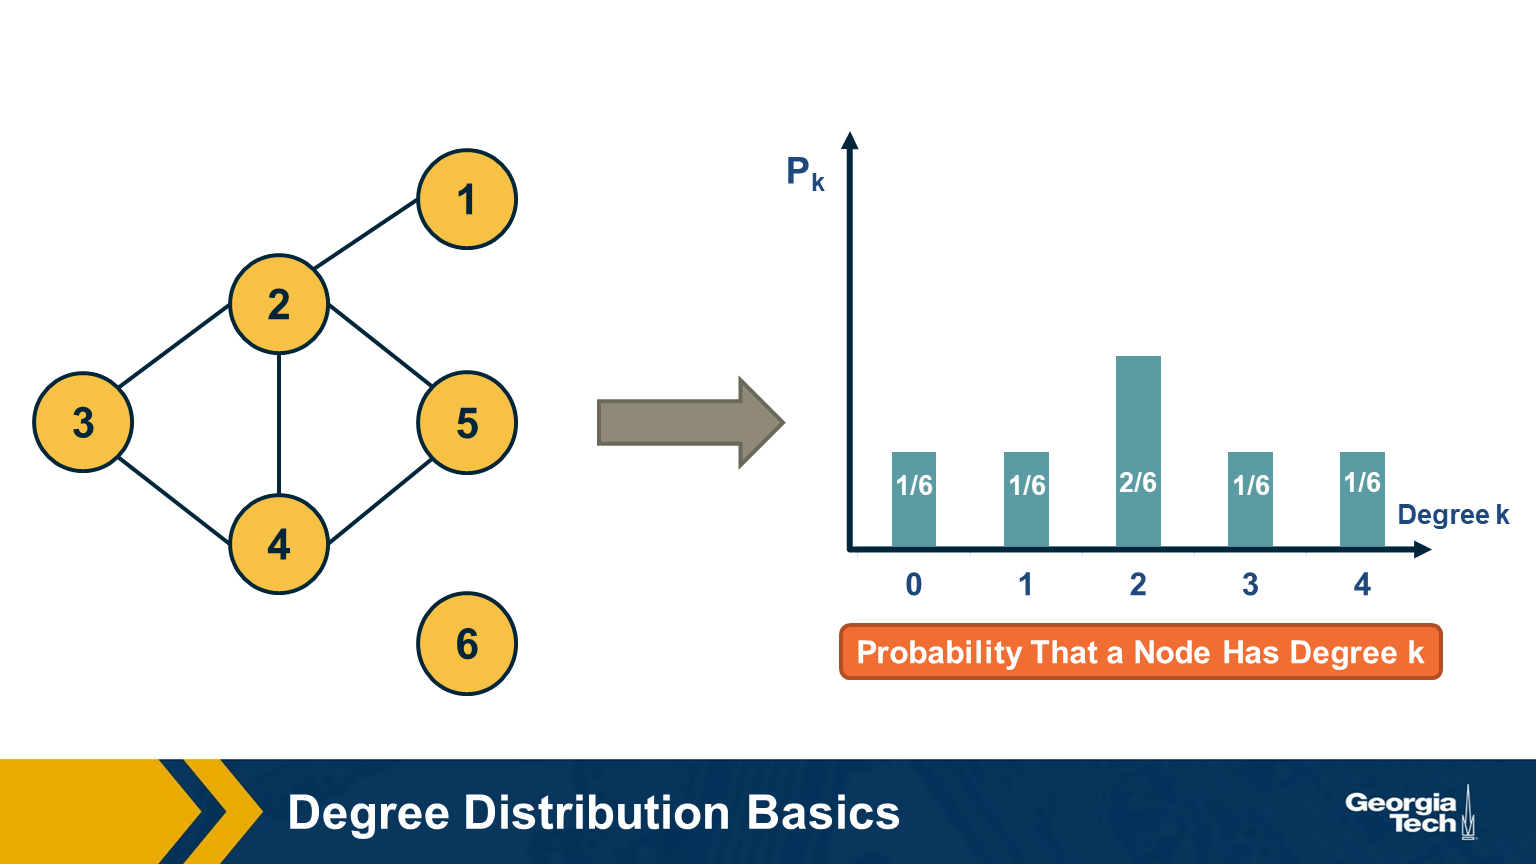
\includegraphics[width=0.75\linewidth]{img/L3.1-DegreeDistro.png}
	\end{center}

\subsubsection{Degree Distribution Moments}
Given the probability distribution of a random variable, we can compute:
\begin{itemize}
	\item \textbf{First Moment (aka mean):} 
			\[ \bar{k} = \sum_{k=0}^{maxdegree} k p_k \]
	\item \textbf{Second Moment:} 
			\[ \bar{k} = \sum_{k=0}^{maxdegree} k^2 p_k \]
	\item \textbf{Variance:} 
			\[ \sigma_{k}^{2} = \overline{k^2} - (\bar{k})^2 \]
\end{itemize}

\subsubsection{Complementary Cumulative Distribution Function}
For larger networks, we usually use the Complementary Cumulative Distribution Function (C-CDF) instead of the empirical probability density function, $p_k$, which shows the probability that the degree is at least k, for any $k>0$.
\[ \overline{P_k} = Prob(degree >= k) = \sum_{x=k}^{\infty} p_x \]

C-CDF plots ($\overline{P_k}$ vs $k$)are often shown with log or log-log scales, since for many networks, the C-CDF decays exponentially (ie $\overline{P_k} = e^{-k\lambda}$) or decays with a power-law of k (ie $\overline{P_k} = ck^{-\alpha}$).

\subsubsection{Friendship Paradox}
\paragraph{Definition:} The average degree of a node's neighbor is higher than the average node degree of the network. Informally, on average, your friend has more friends than you.

\paragraph{Proof: probability that a random edge connects to a node of degree k} Suppose we pick a random edge and randomly select one of the two stubs of the edge. The probability $q_k$ that a randomly chosen stub belongs to a node of degree $k$ is:
\begin{align*} 
	q_k & = (\text{\# of nodes of degree k} \times (\text{probability an edge connects to a specific node of degree k})) \\
	& = (np_k)(\frac{k}{2m}) \\
	& = \frac{kp_k}{2m/n} \\
	& = \frac{kp_k}{\overline{k}} \\
\end{align*}
where $n$ is the number of nodes and $m$ is the number of edges.

The probability that a randomly chosen stub connects to a node of degree k is proportional to both k and the probability that a node has degree k. 

For nodes with degree $k>\overline{k}$, it is more likely to sample one of their stubs than the nodes themselves, and vice versa for nodes with degree $k<\overline{k}$.

\paragraph{Proof: expected value of a neighbor's degree} 

\begin{align*}
	\overline{k_{nn}} & = \sum_{k=0}^{\text{max degree}} k \cdot q_k \\
	& = \sum_{k} k \frac{k p_k}{\overline{k}} \\
	& = \frac{\sum_{k} k^2 p_k}{\overline{k}} \\
	& = \frac{\overline{k^2}}{\overline{k}} \\
	& = \frac{(\overline{k})^2 + (\sigma_k)^2}{\overline{k}} \\
	& = \overline{k} + \frac{\sigma_k^2}{\overline{k}}
\end{align*} 

As long as the variance of the degree distribution is positive, and given our assumption that neighboring nodes have independent degrees, the average neighbor's degree is higher than the average node degree.

\subsubsection{Edge Cases of The Friendship Paradox}
\paragraph{Infinitely large regular network} All nodes have the same degree, and thus the degree variance is 0. The average neighbor's degree is equal to the average node degree.

\paragraph{Infinitely large star network} One hub node at the center, and all peripheral nodes connecting only to the hub. The degree variance diverges as n increases, as does the difference between the average node degree and the average neighbor degree.

\subsubsection{Practical Application of Friendship Paradox}
Suppose we have an epidemic, where a virus is spreading through a social network. Assume there is no natural immunity.  The virus would eventually spread through the entire network. 

Say there is a vaccine: if we can't vaccinate everyone, who should we choose to vaccinate to minimize the spread? We could choose the people with the highest degrees, but that's not always easy to determine in a real-world network. Instead, we could use the "acquaintance immunization" strategy, based on the Friendship Paradox:
\begin{enumerate}
	\item Choose a set of random nodes v
	\item Ask each node in v to identify "most connected" neighbor u
	\item Immunize u
\end{enumerate}

If the network contains any hubs, they will likely be connected to some of the randomly selected nodes.

\subsubsection{The G(n,p) model (ER Graphs)}
The G(n,p) model (aka Gilbert Model, aka Erdos-Renyi (ER) Model) is the simplest random graph model. It is a network with n nodes, where the probability that any two nodes are connected is p.

Assuming no self-edges allowed:
\begin{itemize}
	\item \textbf{Expected number of edges:} $p \cdot \frac{n(n-1)}{2}$
	\item \textbf{Average node degree:} $p \cdot (n-1)$
	\item \textbf{Density of network:} $p$
	\item \textbf{Degree variance:} $p \cdot (1-p) \cdot (n-1)$
\end{itemize}

The degree distribution of the G(n,p) model follows the Binomial(n-1, p) distribution since each node can be connected to $n-1$ other nodes with probability $p$.

The degrees of neighboring nodes are not correlated, so the average neighbor degree of a G(n, p) network is $\overline{k_{nn}} = \overline{k} + (1-p)$, using the binomial distribution. This is $\overline{k_{nn}} = \overline{k} + 1$ using Poisson's approximation when $p \ll 1$ (true for sparse networks). In other words, if we reach a node v by following an edge from another node, the expected value of v’s degree is one more than the average node degree. 

\paragraph{Connected Components in G(n, p)}
There is no guarantee that the G(n, p) model will give a connected network. Note: connection probability is $p \approx \frac{\bar{k}}{n}$.

If $p$ is close to zero, the network consists of many small components. 

When the average degree approaches 1, the largest connected component starts covering a significant fraction of all network nodes, in one "giant component".

\paragraph{Derivation: size of LCC in G(n, p) as a function of p}
Let $S$ be the probability that a node belongs to the LCC, aka the expected value of the fraction of nodes that belong in the LCC.

Then, $\overline{S} = 1-S$ is the probability a node is not in the LCC.

That probability can be written: 
\[ \overline{S} = ((1-p) + p \cdot \overline{S})^{n-1} \]

The first term is for the case that a node v is not connected to another node, and the second term for the case when v is connected to another node that is *not* in the LCC.

Since $p=\frac{\bar{k}}{n-1}$:
\[ \overline{S} = (1- \frac{\bar{k}}{n-1} (1 - \overline{S}))^{n-1} \]

\begin{align*}
\ln \overline{S} & = (n-1) \ln(1-\frac{\bar{k}}{n-1} (1-\overline{S}))\\
	& \approx -(n-1) \frac{\bar{k}}{n-1} (1-\overline{S})
\end{align*}

\[ S = 1 - e^{-\bar{k} S}\]

Phase transition at $\bar{k} = 1$

% TODO

\paragraph{When does G(n,p) have a Single Connected Component?}
How large does $p$ (or $\bar{k}$) need to be so that the LCC covers all nodes?

Suppose that S is the probability that a node belongs in the LCC. 

Then, the probability that a node does NOT connect to ANY node in the LCC:
\[ (1-p)^{Sn} \approx (1-p)^n \]
if  $S \approx 1$.

The expected number of nodes not connecting to LCC:
\[ \overline{k_0} = n (1-p)^n = n(1 - \frac{np}{n})^n \]

Recall that $(1-\frac{x}{n})^{n} \approx e^{-x}$ when $x \ll n$. We assume that the network is sparse ($p \ll 1$): 
\[ \overline{k_0} \approx ne^{-np}\]

If we set $\overline{k_0}$ to less than one node:
\[ ne^{-np} \leq 1\]
\[ -np \leq \ln(\frac{1}{n}) = -\ln n \]
\[p \geq \frac{\ln n}{n}\]
\[\overline{k} = np \geq \ln n\]

which means that when the average degree is higher than the natural logarithm of the network size ($\overline{k} > \ln n$) we expect to have a single connected component.

\subsubsection{Degree Correlations}
So far this lesson, we assumed that the degree of a node does not depend on the degree of its neighbors (ie \textbf{no degree correlations}, aka \textbf{neutral networks}). In mathematical terms, if nodes u and v are connected, we have assumed: 
\[P(\text{degree}(u)|\text{degree}(v)=k') = P(\text{degree}(u)=k|u \text{ connects to another node}) = q_k = p_k \frac{k}{\overline{k}}\]
Note: this probability does not depend on the degree $k'$ of neighbor v.

In general, however, there \emph{are} correlations between the degrees of neighboring nodes, and they are described by the conditional probability distribution:
\[ P(k' | k) = P(\text{a neighbor of a k-degree node has degree k'}) \]

The expected value of this distribution is referred to as the \textbf{average nearest-neighbor degree}, $k_{nn}(k)$, of degree-k nodes:
\[k_{nn}(k) = \sum_{k'} k' \cdot P(k'|k) \]

Recall that we already derived that for a neutral network, $k_{nn}(k)$ is independent of $k$:
\[ k_{nn}(k) = \overline{k} + \frac{\sigma_k^2}{\overline{k}} = \overline{k}_{nn} \] 

In most real networks, $k_{nn}(k)$ \emph{does} depend on $k$.

\paragraph{How To Measure Degree Correlations}
One way to quantify the degree correlations in a network is by modeling (i.e., approximating) the relationship between the average nearest neighbor degree $k_{nn}(k)$ and the degree $k$ with a power law of the form:
\[ k_{nn}(k) \approx a \cdot k^\mu \] 

Then we can estimate the exponent, $\mu$, from the data.
\begin{enumerate}
	\item \textbf{Assortative:} If $\mu>0$, the network is assortative (higher-degree nodes tend to have higher-degree neighbors and lower-degree nodes tend to have lower-degree neighbors).
	\item \textbf{Disassortative:} If $\mu<0$, the network is assortative (higher-degree nodes tend to have lower-degree neighbors).
	\item \textbf{Neutral:} If $\mu$ is statistically not significantly different from zero, we say that the network is neutral.
\end{enumerate}

\subsubsection{Assortative, Neutral, Disassortative Networks}
Examples:
\begin{itemize}
	\item \textbf{Assortative:} Scientific collaboration: nodes (scientists) are connected if they have written at least one research paper together. 
	\item \textbf{Disassortative:} Metabolic network: nodes (metabolites) are connected if they appear on opposite sides of the same chemical reaction in a biological cell.
	\item \textbf{Neutral:} Power grid
\end{itemize}

%-----------------------------------------
% LESSON 3: Reading
\subsection{Reading Notes}

% Ch 3.1
\subsubsection{subsection}
\textbf{}

% Ch 7.1-3

%-----------------------------------------
% END LESSON 3
%-----------------------------------------
%-----------------------------------------
% LESSON 4
%-----------------------------------------
\section{Lesson 4: Random Networks}

Objectives:
\begin{itemize}
	\item Examples of highly skewed degree distributions
	\item Understand the math of power-law distributions and the concept of “scale-free” networks
	\item Learn about models that can generate networks with power-law degree distribution
\end{itemize}

Reading:
\begin{itemize}
	\item Chapter 4 (sections 4.1, 4.2, 4.3, 4.4., 4.7, 4.8, 4.12) from A-L. Barabási, \href{http://networksciencebook.com/}{Network Science}.
	\item Chapter 5 (sections 5.1, 5.2, 5.3) from A-L. Barabási, \href{http://networksciencebook.com/}{Network Science}.
\end{itemize}

%-----------------------------------------
% LESSON 4: LECTURES
\subsection{Lecture Notes}

\subsubsection{Power Law Degree Distribution}
Most real-life networks are highly-skewed, very different from the G(n, p) networks which follow a binomial distribution. Instead, a power-law distribution is a better model.

\begin{itemize}
	\item \textbf{Degree distribution:} $p_k = ck^{-\alpha}$ where $\alpha > 0$
	\item \textbf{Proportionality coefficient:} calculated so that the sum of all degree probabilities is equal to 1 for a given $\alpha$ and a given minimum degree $k_{min}$ .\\ 
\[ c = (\alpha-1) k_{min}^{\alpha-1} \]
	\item Thus, the complete power-law distribution is: 
\[ p_k = \frac{\alpha-1}{k_{min}} (\frac{k}{k_{min}})^{-\alpha} \]
	\item \textbf{C-CDF:} 
\[ P \left[ \text{degree} \geq k \right] = (\frac{k}{k_{min}})^{\alpha-1} \]
\end{itemize}

\subsubsection{Max Degree in Power Law Network}
\[k_{max} = k_{min} n^{\frac{1}{\alpha-1}}\]

This means that the maximum degree in a power-law network increases as a power-law of the network size n. If $\alpha=3$ the maximum degree increases with the square-root of n.

\subsubsection{Failures in Power Law Network}
\textbf{Random Failures}: a fraction of randomly selected nodes are removed from the network

\textbf{Targeted Attacks}: a fraction of nodes with the highest degree are removed from the network

Power-law networks are more robust to random failures than Poisson networks – but they are also more sensitive to targeted attacks than Poisson networks.

\subsubsection{Degree-Preserving Randomization}
To determine whether an interesting property P of a network G is because of its degree distribution or some other property of the network, we can perform randomization of G but preserve the degree of all nodes, then check for property P.

\subsubsection{Average Degree of Nearest Neighbor in Power Law Network}
Recall from lesson 3: for a neutral network (no correlation between the degrees of two connected nodes), the average neighbor degree is: 
\[ \overline{k_n} = \overline{k} + \frac{\sigma_k^2}{\overline{k}}\]

Since power law networks can have very high degree variability (ie $\sigma_k \gg \overline{k}$), then the average neighbor degree can be much higher than the network's average degree (intensifying friendship paradox).

\subsubsection{Generation Models}
\begin{enumerate}
	\item \textbf{Configuration model}: Given the number of nodes, $n$, and degree $k_i$ of each node $i$, the model generates the $n$ nodes, where node $i$ has $k_i$ available "edge stubs". It then continually selects two random available stubs and connects them with an edge until there are no more available stubs. Note that this might create self-loops or multi-edges.
	\item \textbf{Preferential Attachment Model}: (aka PA model aka Barabasi-Albert model) The network grows by one node at each time step. Each time a new node is added, it connects to $m$ existing nodes, chosen randomly but with a non-uniform probability distribution. The probability that the new node at time t will connect to node $i$ is:
\[ \Pi_i (t) = \frac{k_i(t)}{2mt} \]
. New nodes are more likely to connect to nodes with higher degrees. 
	\item \textbf{Link Selection Model} Each time a new node is introduced, select a random link; the new node will connect to one of the two end-points of that link, chosen randomly.
\end{enumerate}

%-----------------------------------------
% LESSON 4: Reading
\subsection{Reading Notes}

% Ch x
\subsubsection{subsection}
\textbf{}

%-----------------------------------------
% END LESSON 4
%-----------------------------------------

%-----------------------------------------
% LESSON 5
%-----------------------------------------
\section{Lesson 5: Network Paths, Clustering, and the "Small World" Property}

Objectives:
\begin{itemize}
	\item \textbf{Network efficiency}: concept + metrics
	\item \textbf{Network clustering}: concept + metrics
	\item Difference between "small-world" networks and random/regular, power-law networks
	\item \textbf{Network motifs}: concept + metrics
	\item Case studies of small-world networks
\end{itemize}

Reading:
\begin{itemize}
	\item Chapter 3, Sections 8-9 from A-L. Barabási, \href{http://networksciencebook.com/}{Network Science}.
	\item Sections 3.1, 3.2, 20.1, 20.2 -  D. Easley and J. Kleinberg, \href{https://www.cs.cornell.edu/home/kleinber/networks-book/networks-book.pdf}{Networks, Crowds and Markets}
%	\item \href{https://doi.org/10.1073/pnas.2133841100\%E2\%80\%8B\%C2\%A0}{Structure and function of the feed-forward loop network motif}, S Mangan and U. Alon, PNAS October 14, 2003 100 (21) 11980-11985
\end{itemize}

%-----------------------------------------
% LESSON 5: LECTURES
\subsection{Lecture Notes}

% L5: 
\subsubsection{Clustering Coefficient}
In social networks, if A is a friend of B and C, then B and C are also likely to be friends with each other. In other words, A, B, and C form a \textbf{“friendship triangle”}. 

To quantify the presence of such triangles, we can use the \textbf{Clustering Coefficient}, defined for node-i with at least two neighbors as the fraction of its neighbors' pairs that are connected.

For an undirected, unweighted network described by adjacency matrix A, the clustering coefficient for node-i is:
\begin{align*}
C_i &= \frac{1/2 \sum_{j,m} A_{i,j}A_{j,m}A_{m,i}}{k_i(k_i-1)/2} \\
	&= \frac{\sum_{j,m} A_{i,j}A_{j,m}A_{m,i}}{k_i(k_i-1)}
\end{align*}
The denominator is the number of neighbor pairs of node-i and the numerator is the number of those pairs that form triangles with node-i.

The clustering coefficient is not well-defined for nodes of degree zero or one.

The clustering coefficient is maximized (1) if node-i and its neighbors form a clique, while the clustering coefficient is minimized (0) if node-i and its neighbors form a star.

To describe the clustering coefficient of the whole network, rather than one specific node, we can plot the average clustering coefficient average clustering coefficient as a function of the degree, k, for all nodes with degree $k>1$.

\subsubsection{Average Clustering and Transitivity Coefficient}
To quantify the degree of clustering in the entire network with a single number, there are two options:
\begin{itemize}
	\item \textbf{Average Clustering Coefficient} for all nodes with degree $>1$.
	\item \textbf{Transitivity (aka Global Clustering Coefficient)}: the fraction of the connected triplets of nodes that form triangles. A \textbf{connected triplet} is an ordered set of three nodes ($ABC$) such that $A$ connects to $B$ and $B$ connects to $C$. An $A$, $B$, $C$ triangle corresponds to three triplets: $ABC$, $BCA$, and $CAB$. The transitivity of the network is defined mathematically as:
\[T = \frac{3 \times \text{number of triangles}}{\text{number of connected triplets}}\]
\end{itemize}

Note: the Transitivity and the Average Clustering Coefficient are two different metrics; while often they can be close, there are certain cases where the two metrics give very different answers. For example: consider a network in which two nodes, $A$ and $B$, are connected to each other as well as all other nodes, with no other links. For a large number of nodes, $n$, the average clustering coefficient approaches $1$: since all nodes other than $A$ and $B$ are only connected to $A$ and $B$, the clustering coefficient of those nodes are $1$. The transitivity, however, is much closer to zero, since any pair of nodes other than $A$ or $B$ forms a connected triplet but not a triangle.

\subsubsection{Clustering in Weighted Networks}
The definition of clustering coefficient can also be generalized for weighted networks as follows. Suppose that $w_{i,j}$ is the weight of the edge between nodes $i$ and $j$.

First, in weighted networks, instead of the degree of a node we often talk about its "strength", defined as the sum of all weights of the node's connections:
\[s_i = \sum_j A_{i,j}w_{i,j}\]

Then, the weighted clustering coefficient of node i is defined as:
\[C_w (i) = \frac{1}{s_i (k_i - 1)} \sum_{j,h} \frac{w_{i,j} + w_{i,h}}{2} A_{i,j} A_{i,h} A_{j,h} \]

The normalization term $\frac{1}{s_i (k_i - 1)}$ is such that the maximum value of the weighted clustering coefficient is one. The product of the three adjacency matrix elements at the right is one only if the nodes $i,j,h$ form a triangle. In that case, that triangle contributes to the clustering coefficient of node-i based on the average weight of the two edges that connect node i with j and h, respectively. Note that the weight between nodes j and h does not matter.

\subsubsection{Clustering in G(n,p) networks}
How large is the expected clustering coefficient at a random ER network?

Recall that any two nodes in that model are connected with the same probability p. So, the probability that a connected triplet A-B-C forms a triangle (A-B-C-A) is also p. Thus, the expected value of the clustering coefficient for any node with more than one connection is p. Similarly, the transitivity (and the average clustering coefficient) of the whole network is also expected to be p.

In $G(n,p)$, the average degree is $\overline{k} = p (n-1)$. If the average degree remains constant, we expect $p$ to drop inversely proportional with $n$ as the network size grows.

Real networks do not show a decreasing trend between the clustering coefficient tand the network size, the way we'd expect if they followed the $G(n,p)$ model. The $G(n,p)$ model predicts negligible clustering, expecially for large and sparse networks. On the contrary, real-world networks have a much higher clustering coefficient than $G(n,p)$, and its magnitude does not seem to depend on the network size.

\subsubsection{Clustering in Regular Networks}
Regular networks typically have a locally clustered topology. The exact value of the clustering coefficient depends on the specific network type but in general, it is fair to say that "regular networks have strong clustering". Further, the clustering coefficient of regular networks is typically independent of their size.

	\begin{center}
		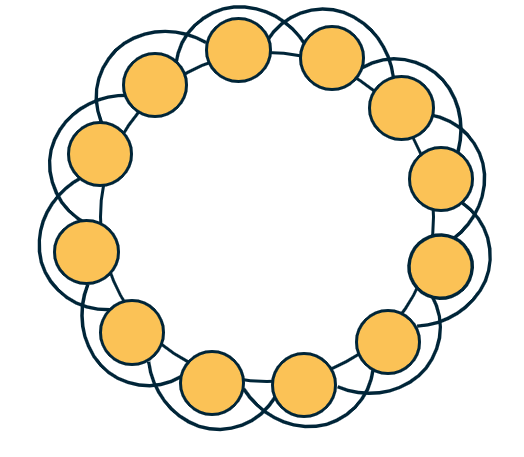
\includegraphics[width=0.75\linewidth]{img/L5.1-RegularNetworkClustering.png}
	\end{center}

To see that, let's consider the common regular network topology shown at the visualization. The n nodes are placed in a circle, and every node is connected to an even number c of the nearest neighbors (c/2 at the left and c/2 at the right). If c=2, this topology is simply a ring network with zero clustering (no triangles). For a higher (even) value of c however, the transitivity coefficient is:
\[ T = \frac{3(c-2)}{4(c-1)} \]
Note this does not depend on the network size. As c increases the transitivity approaches $3/4$.

\subsubsection{Diameter, Characteristic Path Length, and Network Efficiency}
The notion of small-world networks depends on two concepts: how clustered the network is (see above) and how short the paths between network nodes are.

If a network forms a connected component, we can compute a shortest-path length, $d_{i,j}$ between any two nodes $i$ and $j$. One way to summarize these distances for the entire network is to simply take the average such distance across all distinct node pairs. This metric L is referred to as \textbf{Average (shortest) Path Length (APL)} or \textbf{Characteristic Path Length (CPL)} of the network. For an undirected and connected network of n nodes, we define L as:
\[ L = \frac{2}{n(n-1)} \sum_{i<j} d_{i,j} \]

A related metric is the harmonic mean of the shortest-path lengths across all distinct node pairs, referred to as the \textbf{efficiency} of the network:
\[ E = \frac{2}{n(n-1)} \sum_{i<j} \frac{1}{d_{i,j}} \]
The efficiency varies between 0 and 1.

Another metric that is often used to quantify the distance between network nodes is the diameter, which is defined as the maximum shortest-path distance across all node pairs:
\[ D = max_{i<j} d_{i,j}\]

A more informative description is the distribution of the shortest-path lengths across all distinct node pairs.

\subsubsection{Diameter and CPL of G(n,p) Networks}
\paragraph{Approximation of diameter}
We can derive an approximate expression for the diameter of the $G(n,p)$ network as follows:

Suppose the average degree is:
\[ \overline{k} = (n-1) p > 1 \]
so that the network has a giant connected component. We will further assume that the topology of the network is a tree.

Start from node $i$. Within one hop away from that node, we expect to visit $\overline{k}$ nodes. Within two hops, we expect to visit approximately $\overline{k}^2$ nodes. Similarly, after $s$ hops, we expect to visit approximately $(\overline{k})^s$ nodes.

The total number of nodes in the network is $n$,  and we expect to visit all of them with the maximum number of hops that is possible, which is the network diameter D. So, $n \approx (\overline{k})^D$. Solving for D:
\[ D \approx \frac{\ln n}{\ln \overline{k}} \]

In a random network, even the longest shortest-paths are expected to grow very slowly (logarithmically) with the size of the network.

\paragraph{More accurate estimates of diameter for a sparse G(n,p) network}
As $k$ approaches 1 from above (ie the network is still expected to have a large connected component), the diameter is expected to be:
\[ D \approx 3 \frac{\ln n}{\ln \overline{k}} \]

\paragraph{More accurate estimates of diameter for a dense G(n,p) network}
For dense networks, a good approximation for the diameter is:
\[ D \approx \frac{\ln n}{\ln \overline{k}} + \frac{2 \ln n}{\overline{k}} + \ln n \frac{\ln \overline{k}}{(\overline{k})^2 } \]

\paragraph{Note} the diameter is still increasing with the logarithm of the network size, so the main qualitative conclusion remains: the diameter of G(n,p) networks increases very slowly (logarithmically) with the number of nodes – and so the CPL cannot increase faster than that either.

\subsubsection{Diameter and Efficiency of G(n,p) Versus Regular Networks}
In one-dimensional lattices, each node has two neighbors, and the lattice is a line network of n nodes -- so the diameter increases linearly with n.

In two dimensions, each node has 4 neighbors, and the lattice is a square with $\sqrt{n}$ nodes on each side, so the diameter increases as $O(n^{1/2})$.

In lattice networks, the diameter and CPL grows as a power law of the network size, which grows much faster than a logarithmic function.

\subsubsection{What is a "small-world" network?}
Real world networks often have:
\begin{itemize}
	\item Strong clustering: similar to that of lattice networks with the same average degree
	\item Short paths: similar to the CPL and diameter of G(n,p) networks with the same size n and density p
\end{itemize}
These are referred to as \textbf{small-world networks}. They are small in the sense that the shortest path increases logarithmically as a function of the size of the network.

\paragraph{Watts Strogatz Model} 
Start with regular network. With small probability $p$, choose an edge and reassign one of the stubs to a new randomly chosen node. As rewiring probability approaches 1, the network becomes more random.

\subsubsection{Clustering in PA Model}
\paragraph{Preferential attachment model:}

TODO

\subsubsection{Length of Shortest Paths in PA Model}
TODO

\subsubsection{Path Lengths in Power-law Networks}
TODO

\subsubsection{Directed Subgraph Connectivity Patterns}
	\begin{center}
		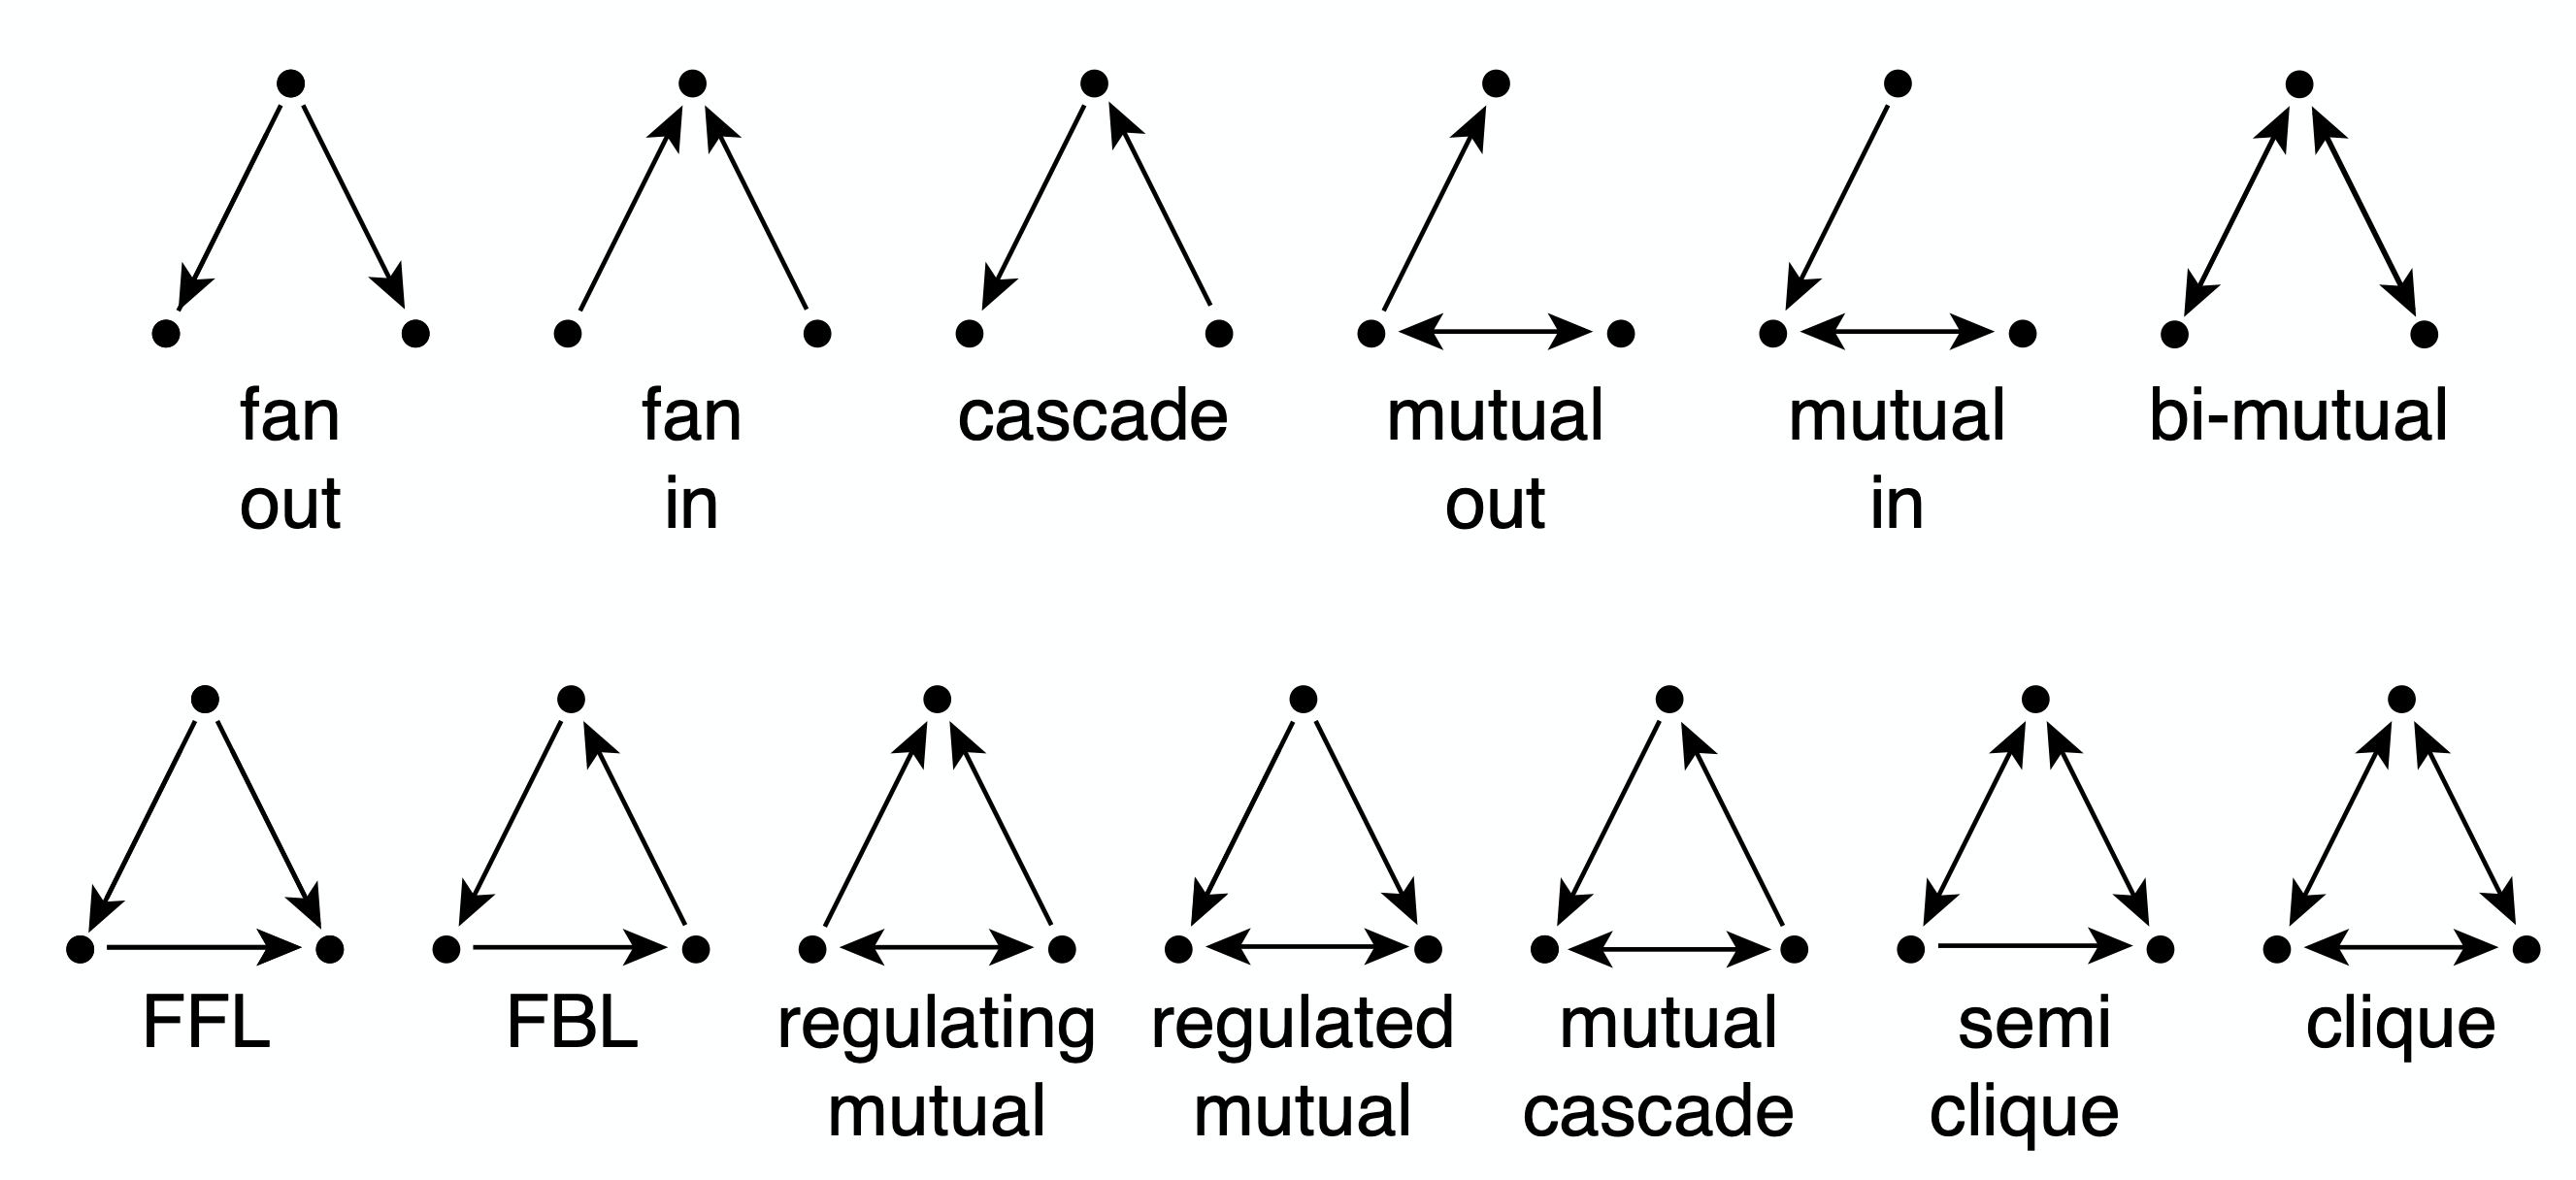
\includegraphics[width=0.75\linewidth]{img/L5.2-DirectedSubgraphConnectivity.PNG}
	\end{center}
This figure shows all 13 types of connection patterns between three weakly connected network nodes. Each of these patterns will be referred to as \textbf{network motifs}.

\subsubsection{Statistical Test For The Frequency of a Network Motif}
What does it mean when a specific network motif occurs very frequently? Or the opposite, what does it mean when a network motif occurs much less frequently than expected based on chance?

TODO

\subsubsection{Frequent Motifs and Their Function}
\textbf{}

%-----------------------------------------
% LESSON 5: Reading
\subsection{Reading Notes}

% Ch x
\subsubsection{subsection}
\subsubsection{}
\textbf{}

%-----------------------------------------
% END LESSON 5
%-----------------------------------------


%-----------------------------------------
% LESSON 6:
%-----------------------------------------
\section{Lesson 6: Centrality Metrics and Network-Core Metrics and Algorithms}

Objectives:
\begin{itemize}
	\item Understand the problem of finding individually important nodes/edges or groups of important nodes/edges
	\item Define and analyze common centrality metrics
	\item Define and analyze common "network core" metrics
	\item Learn how to apply centrality metrics and core identification algorithms through case studies
\end{itemize}

Reading:
\begin{itemize}
	\item Chapter 7, Sections 1-8 from M.E.J. Newman, \href{https://www.amazon.com/Networks-Mark-Newman/dp/0198805098/}{Networks: An Introduction}.
	\item Section 14.3 - D. Easley and J. Kleinberg, \href{https://www.cs.cornell.edu/home/kleinber/networks-book/networks-book.pdf}{Networks, Crowds and Markets}
	\item (Recommended) Sabrin, K, Dovrolis, C. \href{https://www.cambridge.org/core/journals/network-science/article/hourglass-effect-in-hierarchical-dependency-networks/DDBCA83D16CA74B827DAB66A98CC906A}{The Hourglass Effect in Hierarchical Dependency Networks}, Journal of Network Science, (2017)
	\item (Recommended) Faskowitz, J., Yan, X., Zuo, X. et al. \href{https://www.nature.com/articles/s41598-018-31202-1}{Weighted Stochastic Block Models of the Human Connectome across the Life Span}. Sci Rep 8, 12997 (2018).
\end{itemize}

%-----------------------------------------
% LESSON 6: LECTURES
\subsection{Lecture Notes}

% Lx: Module 1
\subsubsection{Degree, Eigenvector and The Katz Centrality}
\paragraph{Degree and Strength Centrality} 
The simplest way to define the importance of a network node is based on its number of connections - the more connections a node has, the more important it is. So, the \textbf{degree centrality} of a node is simply the degree of that node.

For weighted networks, the corresponding metric is the sum of the weights of all edges of that node, i.e., the \textbf{strength} of that node.

For directed networks, we can separate between in-degree and out-degree centrality.

One problem with this definition of centrality is that it only captures the "local role" of a node in the network. A node might have many connections in an isolated cluster, or you could have a very important node that only has a few direct connections but connects two large groups that are otherwise disconnected. This centrality is also easy to manipulate.

\paragraph{Eigenvector Centrality}
A better centrality metric is to consider not only the number of neighbors of a node -- but also the centrality of those neighbors. A node is more central when its neighbors are also more central.

Suppose that we are given an undirected network with adjacency matrix $A$. The centrality of node $i$ is defined:
\[ v_i = \frac{1}{\lambda} \sum_{j} A_{i,j} v_j \]

The $\frac{1}{\lambda}$ term can be thought of as a normalization constant for now. Note that the centrality of a node is the (normalized) sum of the centralities of all its neighbors.

This can also be written in matrix form as 
\[ \lambda v = A v\]
where v is the vector of all node centralities. Notice that this is the same as the definition of the eigenvector of A: $\lambda$ is the corresponding eigenvalue for eigenvector $v$. Thus, we refer to this centrality metric as "eigenvector centrality".

We wish to have non-negative centralities. In other words, the eigenvector $v$ corresponding to eigenvalue $\lambda$ should consist of non-negative entries. It can be shown (using the Perron–Frobenius theorem) that using the largest eigenvalue of $A$ satisfies this requirement.

\paragraph{The Katz Centrality}
The Katz centrality metric is a variation of eigenvector centrality that is more appropriate for directed networks.

The eigenvector centrality may be zero even for nodes with non-zero in-degree and out-degree,  and so Katz starts from the same equation as eigenvector centrality but it also assigns a small centrality $\beta$ to every node, so the definition of the Katz centrality of node $i$ is:
\[ v_i = \beta + \frac{1}{\lambda} \sum_{j} A_{i,j} v_j \]
where the summation is over all nodes $j$ that connect with $i$.

Given that we are only interested in the relative magnitude of the centrality values, we can arbitrarily assign $\beta = 1$.

Rewriting the definition in matrix form:
\[ v = (I - \frac{1}{\lambda})^{-1} \cdot \textbf{1} \]
where \textbf{1} is an $n \times 1$ vector of all ones.

The value of $\lambda$ controls the relative magnitude between the constant centrality $\beta$ we assign to each node and the centrality that each node derives from its neighbors. If $\lambda$ is very large, then the former term dominates and all nodes have roughly the same centrality. If $\lambda$ is too small, on the other hand, the Katz centralities may diverge. This is the case when the determinant of the matrix $(I - \frac{1}{\lambda} A)$ is zero, which happens when $\lambda$ is equal to an eigenvalue of A. To avoid this divergence, the value of $\lambda$ is typically constrained to be larger than the maximum eigenvalue of A.

\subsubsection{PageRank Centrality}
PageRank is a famous centrality metric because it was the main algorithm that made Google the most successful search engine back in the late 1990s.

PageRank is only a slight modification of the Katz centrality metric. It is based on the following idea: if a node j points to a node i (thus $A_{i,j}=1$), and node j has $k_{j, \text{out}}$ outgoing connections, then the centrality of node j should be "split" amoung those $k_{j, \text{out}}$ neighbors. In other words, the "wealth" of node j should not be just inherited by all nodes it points to, but rather, the "wealth" of node j should be split among those nodes.

So, the PageRank centrality becomes:
\[ v_i = \beta  + \frac{1}{\lambda} \sum_{j} A_{i,j} \frac{v_j}{k_{j, \text{out}}} \]
where the summation is over all nodes j that point to i (and thus, $k_{j, \text{out}}$ is non-zero).

In matrix form when $\beta=1$:
\[ v = (I - \frac{1}{\lambda}AD)^{-1} \cdot \textbf{1} \]
where $D$ is a diagonal $n\times n$ matrix in which the jth element is $\frac{1}{k_{j, \text{out}}}$ if $k_{j, \text{out}}$ is non-zero.

Undirected networks are typically transformed to directed networks by replacing each undirected edge with two directed edges.

In practice, the computation of both Katz and PageRank centralities is performed numerically, using a power-iteration method that iterates the computation of the centrality values until those values converge. Typical values for $\frac{1}{\lambda}$ and $\beta$ are $0.85$ and $(1 - \frac{1}{\lambda})/n$, respectively. It is theoretically possible that the Katz and PageRank centrality computations do not converge if $\lambda$ is too low.

\subsubsection{Closeness Centrality and Harmonic Centrality}
The previous centrality metrics are all based on the direct connections of a node. Another group of centrality metrics focuses on network paths. Paths represent ”routes” over which something is transferred through a network. Consequently, another way to think about the centrality of a node is based on how good the routes are of that node to the rest of the network.

\paragraph{Closeness Centrality} A commonly used path-based metric is closeness centrality. It is based on the length (number of hops) of the shortest-path between a node i and a node j, denoted by $d_{i,j}$.  The closeness centrality of node i is defined as the inverse of the average shortest path length $d_{i,j}$, across all nodes j that i connects to:
\[ v_i = \frac{n-1}{\sum_j d_{i,j}} \]
where j is any node in the same connected component with i, and n is the number of nodes in that connected component (including i). If the network is directed, then we typically focus on shortest-paths from any node j to node i (i.e., incoming paths to i). The range of closeness centrality values is limited between 0 and 1.

The closeness centrality has some shortcomings, including the fact that it does not consider all network nodes – only nodes that are in the same connected component with i. So an isolated cluster of nodes can have high closeness centrality values (close to 1) even though those nodes are not even connected to most other nodes.

\paragraph{Harmonic Centrality}
An improved metric is harmonic centrality, defined as:
\[ v_i = \sum_{j \neq i} \frac{1}{d_{i,j}} \] 
Here, if nodes i and j cannot reach other, the corresponding distance can be thought of as infinite, and thus the term $ \frac{1}{d_{i,j}} $ is 0.

Sometimes, the harmonic centrality is normalized by $\frac{1}{n-1}$, but that does not affect the relative ordering of node centralities.

\subsubsection{Betweenness Centrality Variants}
In some network analysis applications, the importance of a node is associated with how many paths go through a node: the more routes go through a node, the more central that node is.

\paragraph{Shortest-path Betweenness Centrality}
Consider any two nodes s (source) and t (target) in the same connected component, and let us define the number of shortest-paths between these two nodes as $n_{s,t}$. Also, suppose that the subset of these paths that traverses node i is $n_{s,t}(i)$ where i is different from s and t.

The shortest-path betweenness centrality of node i is:
\[ v_i = \sum_{s,t \neq i} \frac{n_{s,t}(i)}{n_{s,t}} \] 
If s and t are the same, then $n_{s,t}=1$.

The previous metric is often normalized by its maximum possible value so that the centrality values are between 0 and 1. This is not necessary however given that we only care about the relative magnitude of centralities.

For weighted networks, the shortest-paths can be computed using Dijkstra’s algorithm for weighted networks.

There are many variants on the betweenness centrality metric, depending on the kind of paths used.
\begin{itemize}
	\item \textbf{Flow Betweenness Centrality}: compute the max-flow from any source node s to any target node t, and then replace the fraction $\frac{n_{s,t}(i)}{n_{s,t}}$ with the fraction of the max-flow that traverses node i.
	\item \textbf{Random-Walk Betweenness Centrality}: number of random walks from node s to node t that traverse node i.
\end{itemize}

\paragraph{Edge Centrality Metrics}
In some cases, we are interested in the centrality of edges, rather than nodes. One such metric is the \textbf{edge betweenness centrality}. The definition is the same as for node betweenness centrality – but instead of considering the fraction of paths that traverse a node i, we consider the fraction of that traverse an edge (i,j). These paths can be shortest-paths or any other well-defined set of paths, as we discussed on the previous page.

Another way to define the centrality of an edge is to quantify the impact of its removal. For instance, one could measure the increase in the Characteristic Path Length (CPL, see Lesson-5) after removing edge (i,j) – the higher that CPL increase is, the more important that edge is for the network.
 
\subsubsection{Path Centrality For Directed Acyclic Graphs}

In directed acyclic graphs (DAGs), we can consider all paths from the set of sources to the set of targets. Each source-target path (ST-path) represents one \textbf{"dependency chain"} through which that target depends on the corresponding source.

The path centrality of a node (including sources or targets) is defined as the total number of source-target paths that traverse that node.

It can be easily shown that the path centrality of node-i is the product of the number of paths from all sources to node-i, times the number of paths from node-i to all targets. The former term can be thought of as the \textbf{"complexity"} of node-i, while the second term can be thought of as the \textbf{"generality"} of node-i.


\subsubsection{The Notion of "Node Importance"}
We've defined a number of centrality metrics now -- which metric should we use for each network analysis application? To choose the right metric, it is important to understand the notion of \textbf{"node importance"} that each of these centrality metrics focuses on.

\begin{itemize}
	\item \textbf{Degree (or strength) centrality}: appropriate when we are interested in the number or weight of direct connections of each node, eg finding the person with the most friends in a social network.
	\item \textbf{Eigenvector/Katz/PageRank centrality}: appropriate when we are mostly interested in the number of connections with other well-connected nodes. For undirected networks, it is better to use Eigenvector centrality because it does not depend on any parameters. For directed networks, use Katz or PageRank depending on whether it makes sense to split the centrality of a node among its outgoing connections.
	\item \textbf{Closeness (or harmonic) centrality}: appropriate when we are interested in how fast a node can reach every other node. If the network includes multiple connected components, it is better to use harmonic centrality.
	\item \textbf{Betweenness centrality}: appropriate in problems that involve some form of transfer through a network, and the importance of a node relates to whether that node is in the route of such transfers. You should use a betweenness centrality that captures correctly the type of routes used in that network. For instance, if the network uses shortest-path routes, it makes sense to use shortest-path betweenness centrality. If however, the network uses equally all possible routes between each pair of nodes, the path centrality may be a more appropriate metric.
\end{itemize}

\subsubsection{k-core Decomposition}
Sometimes instead of trying to rank individual nodes in terms of centrality, we are interested in identifying the most important group of nodes in the network. There are different ways to think about the importance of groups of nodes. One of them is based on the notion of \textbf{k-core}.

A k-core (or "core of order-k") is a maximal subset of nodes such that each node in that subset is connected to at least k others in that subset.

\begin{center}
	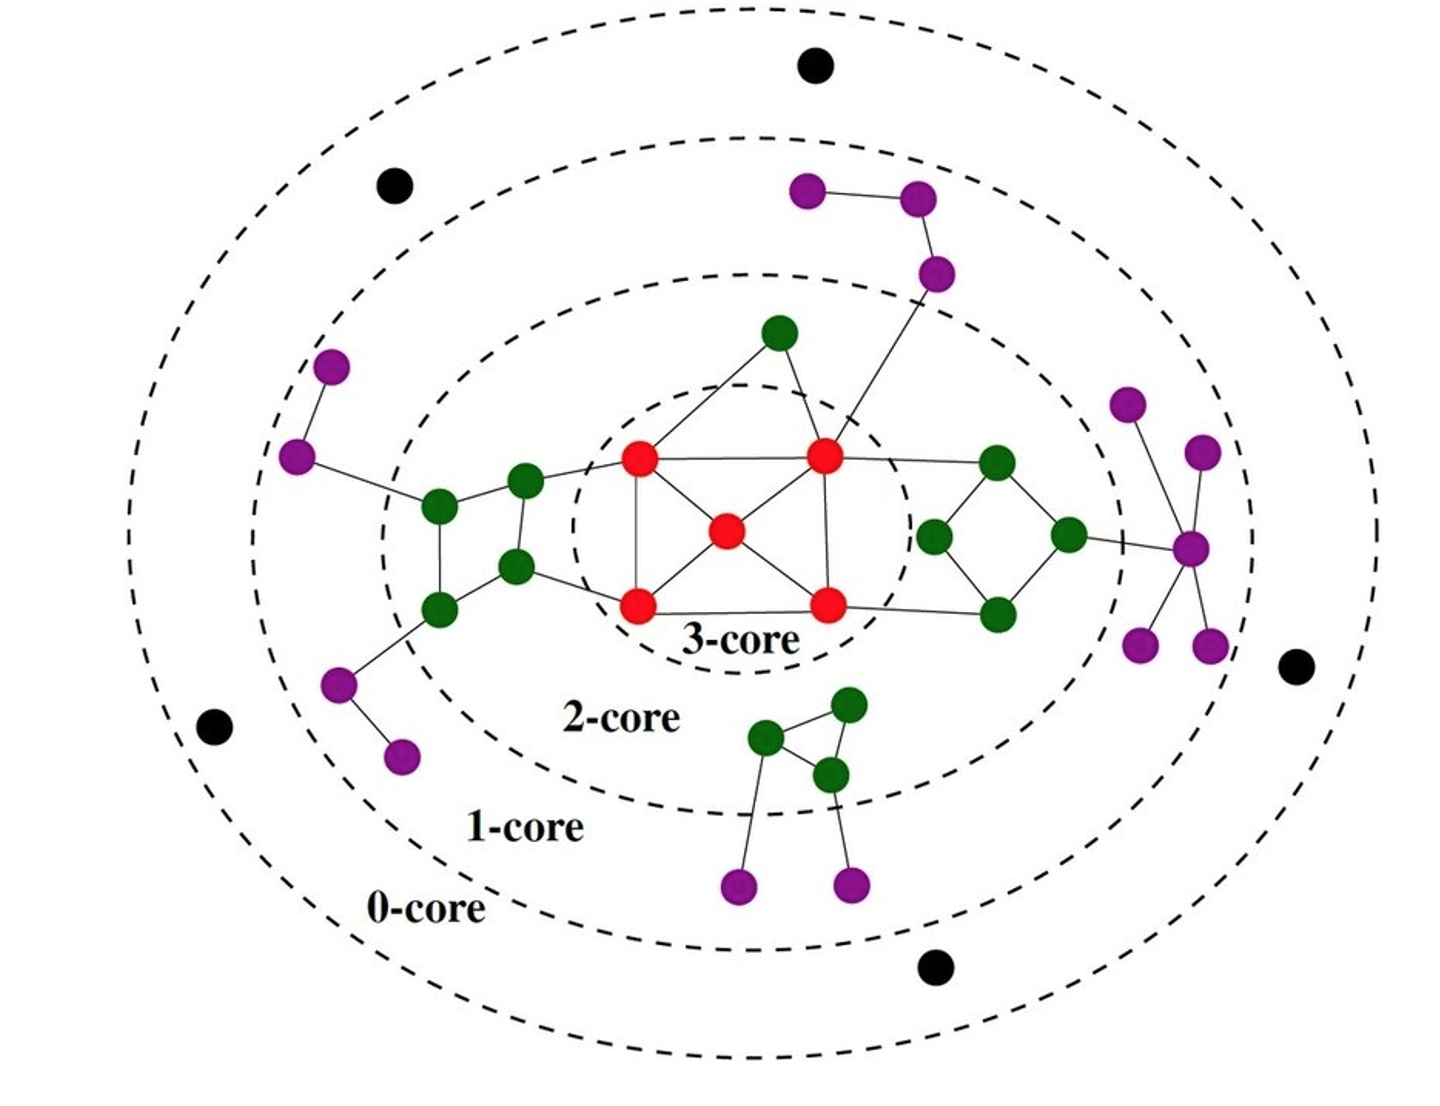
\includegraphics[width=0.75\linewidth]{img/L6.1-kCoreDecomposition.PNG}
\end{center}
The visualization shows a network in which the red nodes belong to a core of order-3 (the highest order in this example), the green and red nodes form a core of order-2,  while all nodes (except the black) form a core of order-1.

Note that there is a purple node with degree=5, but its highest order is 1 because all its connections except one are to nodes of degree-1. Similarly, there are green nodes of degree-3 that are in the 2-core set.

\paragraph{k-core decomposition} is a simple algorithm which can associate each node with the highest k-core order that that node belongs to.

Algorithm:
\begin{enumerate}
	\item Iteratively remove all nodes of degree k, for $k=0, 1, 2...$.
	\item If, during the removal of nodes of degree k, some higher-degree nodes lose connections and become degree k, remove those nodes too and add them to the k-core.
	\item Terminate when all nodes have been removed.
\end{enumerate}

We can think about k-cores as successive layers of an onion, where $k=1$ corresponds to the external layer of the onion, and the highest k corresponds to the "heart" of the onion. The k-core decomposition process gradually peels off the network layer by layer until it reaches its most internal group of nodes.

The nodes in the maximum core order are considered as the most well-connected group of nodes in the network.

\paragraph{k-shell:} the subgraph induced by nodes in the k-core that are not in the (k+1)-core. For example, the green nodes in the visualization form the 2-shell.

\subsubsection{Core-Periphery Structure}
Networks with a core-periphery structure can be partitioned in two groups: 
\begin{itemize}
	\item core nodes 
	\item periphery nodes
\end{itemize}

Core nodes are very densely connected to each other and the rest of the network. Periphery nodes are well-connected only to core nodes.

\subsubsection{Rich-Club Set of Nodes}
A common approach for the detection of core-periphery structure is referred to as the \textbf{rich-club} of a network.

For undirected networks, suppose that the number of nodes with degree greater than k is $n_k$. Let $e_k$ be the number of edges between those nodes. The maximum number of possible edges between those nodes is $\frac{n_k(n_k - 1)}{2}$. The "rich-club coefficient" for degree k is defined as:
\[ \phi (k) = \frac{2e_k}{n_k(n_k - 1)} \]
and quantifies the density of connections between nodes of degree greater than k.

To determine whether the value of $\phi (k)$ is statistically significant for a given k, generate an ensemble of random networks with the same number of nodes and degree distribution (see lesson 4). These random networks represent our \textbf{null model}. Compute the average value of $\phi (k)$ across all random networks for each k.

If the rich-club coefficient for degree k in the given network is much larger than the corresponding coefficient in the null model, we can mark that value of k as statistically significant for the existence of a rich-club. If there is at least one such statistically significant value of k, we conclude that the network includes a rich-club -- the set of nodes with degree greater than k. If there are multiple such values of k, the rich-club nodes can be identified based on the value of k for which we have the largest difference between the rich-club coefficient in the real network versus the null model (even though there is some variation about this in the literature).

\subsubsection{Core Set of Nodes in DAGs}
A path-based approach to identify a group of core nodes in a network is referred to as the "$\tau$-core".

We define that a node v \textbf{"covers"} a path p when v is traversed by p. 

The $\tau$-core is defined: given a set of network paths P we are interested in, what is the minimal set of nodes that can cover at least a fraction $\tau$ of all paths in P?

In the context of DAGs, the set P can be the ST-paths from the set of all sources to all targets.

The rationale for covering only a fraction  of paths (say 90\%) instead of all paths is because in many real networks there are some ST-paths that do not traverse any intermediate nodes.

The problem of computing the the "$\tau$-core" has been shown to be NP-Complete in the following paper: Sabrin, Kaeser M., and Constantine Dovrolis. "The hourglass effect in hierarchical dependency networks."

\subsubsection{Applications}
\begin{enumerate}
	\item \textbf{GOT Network}: interactions of characters in Game of Thrones.
\end{enumerate}

%-----------------------------------------
% LESSON 6: Reading
\subsection{Reading Notes}

% Ch x
\subsubsection{subsection}
\textbf{}

%-----------------------------------------
% END LESSON 6
%-----------------------------------------


%-----------------------------------------
% LESSON 7
%-----------------------------------------
\section{Lesson 7: Modularity and Community Detection}

Objectives:
\begin{itemize}
	\item Understand the community detection problem
	\item Utilize the modularity metric and appreciate its limitations
	\item Analyze and deploy algorithms for community detection
	\item Understand the notion of hierarchical modularity
\end{itemize}

Reading:
\begin{itemize}
	\item Chapter-9 from A-L. Barabási, \href{http://networksciencebook.com/}{Network Science}.
\end{itemize}

%-----------------------------------------
% LESSON 7: LECTURES
\subsection{Lecture Notes}

\subsubsection{The Graph Partitioning Problem}
\textbf{Graph Partitioning} is a classical problem in computer science. Given a graph, how would we partition the nodes in two non-overlapping sets of the same size so that we minimize the number of edges between the two sets? This is also known as the \textbf{Minimum Bisection Problem}.

We can also state more general versions of this problem in which we partition the network into K non-overlapping sets of the same size, where $K>2$ is a given constant.

The graph partitioning problem is NP-complete, so we only have approximate solutions. The \textbf{Kerninghan-Lin Algorithm} iteratively switches a node from one partition with a node from the other partition, selecting whichever pair causes the largest reduction in the number of edges that cut across the partition.

\subsubsection{Network Community Detection}
In the \textbf{Community Detection Problem}, we also need to partition the network into a set of non-overlapping clusters or communities, but this time we do not know a priori the number of sets, and they do not necessarily need to be the same size.

What are the key properties that define a community? Loosely speaking, the nodes should form a densely connected sub-graph. But this is not a mathematically precise definition, since we did not define how dense the sub-graph should be.

One extreme is to use a maximally sized clique, ie the largest subgraph that is still complete. This is a stringent definition, doesn't capture the fact that sometimes there might be missing edges between nodes in a community.

Instead, we could think of a community as an approximate clique: a subgraph in which the number of internal edges (edges between nodes of the subgraph) is much greater than the number of external edges (edges between a node of the subgraph and a node in the rest of the graph). This is still a loose definition.

Another way to think about network communities is through the adjacency matrix. Suppose a network has k non-overlapping groups of nodes of different sizes, such that the density of internal connections is much greater than the density of external connections. If we reorder the adjacency matrix so that the nodes of its group appear in consecutive rows, we will observe that the adjacency matrix contains much denser submatrices for each community.

Let's define communities better:
\begin{itemize}
	\item Is every node required to belong to a community?
	\item Are communities necessarily non-overlapping? Can a node belong to more than one community?
	\item What if there are no real communities in the network? What if the network is randomly formed?
\end{itemize}

\subsubsection{Community Detection Based on Edge Centrality Metrics}
A family of algorithms for community detection is based on hierarchical clustering. The goal of such approaches is to create a tree structure, or "dendrogram", that shows how the nodes of the network can iteratively split in a top-down manner into smaller and smaller communities (\textbf{"divisive hierarchical clustering"}) - or how the nodes of the network can be iteratively merged in a bottom-up manner into larger and larger communities (\textbf{"agglomerative hierarchical clustering"}).

Starting with divisive algorithms: we first need a metric to select edges that fall between communities - the iterative removal of such edges will gradually result in smaller and smaller communities.

One such metric is the edge (shortest path) betweenness centrality, ie the fraction of shortest paths, across all pairs of terminal nodes, that traverses a given edge  (see lesson 6). Removing the edge with the maximum centrality value will partition the network into two communities. We can then recompute the betweenness centrality for each remaining edge, and repeat the process to identify the next smaller communities.  This algorithm is referred to as \textbf{"Girvan-Newman"} in the literature.

Another edge centrality metric that can be used for the same purpose is the random walk betweenness centrality. Here, instead of following shortest paths from a node u to a node v, we compute the probability that a random walk that starts from u and terminates at v traverses each edge e. The edge with the highest such centrality is removed first.

Note that the computational complexity of such algorithms depends on the algorithm we use for the computation of the centrality metric. 
\begin{itemize}
	\item For betweenness centrality, that computation can be performed in $O(LN)$, where $L$ is the number of edges and $N$ is the number of nodes. 
	\item Given that we remove one edge each time, and need to recompute the centrality of the remaining edges in each iteration, the computational complexity of the Girvan-Newman algorithm is $O(L^2 N)$. In sparse networks the number of edges is in the same order with the number of nodes, and so the Girvan-Newman algorithm runs in $O(N^3)$.
\end{itemize}

\subsubsection{Divisive Hierarchical Community Detection}
To illustrate the iterative top-down process followed by divisive hierarchical community detection algorithms, let us focus on the edge betweenness centrality metric. The Girvan-Newman algorithm uses that metric to remove a single edge in each iteration – the edge with the highest edge betweenness centrality. 

The value of the edge betweenness centrality of the remaining edges has to be re-computed because the set of shortest paths changes in each iteration.

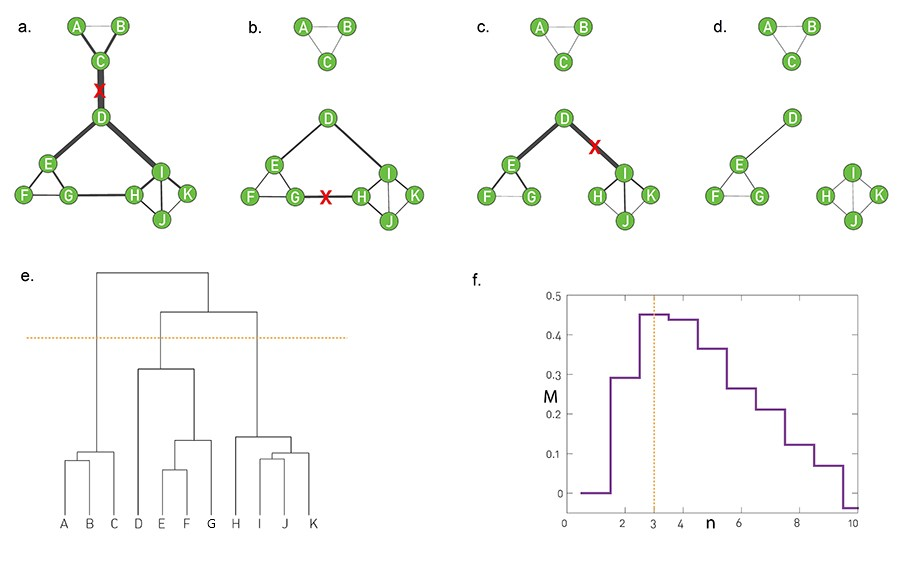
\includegraphics[width=0.9\linewidth]{img/L7.1-DivisiveHierarchicalCommunityDetection.jpg}

Note that a hierarchical clustering process does NOT tell us what is the best set of communities – each horizontal cut of the dendrogram corresponds to a different set of communities. So we clearly need an additional objective or criterion to select the best such set of communities. Such a metric, called modularity M, is shown in the visualization (f), which suggests we cut the dendrogram at the point of three communities (yellow line).

This algorithm always detect communities in a given network. So, even a random network can be split in this hierarchical manner, even though the resulting communities may not have any statistical significance.    

\subsubsection{Agglomerative Hierarchical Clustering Approaches - Node Similarity Metric}
Agglomerative hierarchical clustering algorithms are bottom-up approaches. We start at the dendogram leaves, one for each node. In each iteration, we decide which nodes to merge and build the dendrogram up. Ideally, the merged nodes should belong to the same community, so we need a metric that quantifies the likelihood of two nodes belonging to the same community.

If two nodes, i and j, belong to the same community, we expect they will both be connected to several other nodes of the same community, so we expect them to have a large number of common neighbors, relative to their degree.

We define a similarity metric between any pair of nodes i and j:
\[ S_{i,j} = \frac{N_{i,j} + A_{i,j}}{\min\{k_i, k_j\}} \]
where $N_{i,j}$ is the number of common neighbors of i and j, $A_{i,j}$ is the adjacency matrix element for the two nodes (1 if connected, 0 otherwise), and $k_i$ is the degree of node i.

Note that $S_{i,j} = 1$ if the two nodes are connected with each other and every neighbor of the lower-degree node is also a neighbor of the other node.  On the other hand, $S_{i,j} = 0$ when the two nodes are not connected to each other, and do not have any common neighbors.

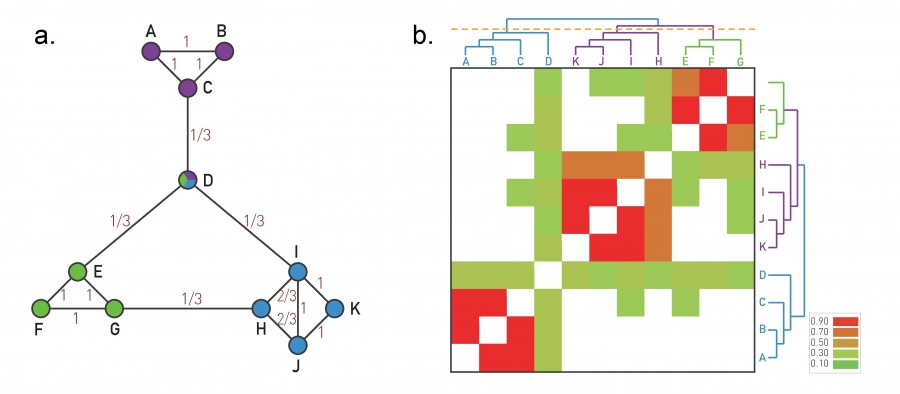
\includegraphics[width=0.9\linewidth]{img/L7.2-AgglomerativeHierarchicalCommunityDetection.jpg}

The visualization on the left shows the node similarity value for each pair of connected nodes. The visualization on the rights shows the color-coded node similarity matrix, for every pair of nodes (even if they are not connected). Note that three groups of nodes emerge with higher similarity values: (A, B, C), (H,I,J,K) and (E,F,G). Node D on the other hand has a lower similarity with any other node, and it appears to be a "connector" between the three communities.

\subsubsection{Hierarchical Clustering Approaches - Group Similarity}
Three ways to compute the similarity between two groups of nodes:
\begin{itemize}
	\item \textbf{Single Linkage:} the similarity of groups 1 and 2 is determined by the minimum distance (i.e., maximum similarity) across all pairs of nodes in groups 1 and 2.  
	\item \textbf{Complete Linkage:} the similarity of groups 1 and 2 is determined by the maximum distance (i.e., minimum similarity) across all pairs of nodes in groups 1 and 2. 
	\item \textbf{Average Linkage:} the similarity of groups 1 and 2 is determined by the average distance (i.e., average similarity) across all pairs of nodes in groups 1 and 2.
\end{itemize}

Average linkage is the most commonly used metric.

\paragraph{Where To Cut The Dendrogram}
Now we can design an iterative algorithm, known as the \textbf{Ravasz algorithm}, to compute a hierarchical clustering dendrogram in a bottom-up manner:
\begin{enumerate}
	\item Start with each node represented as a leaf of the dendrogram. Compute the matrix of $N^2$ pairwise node similarities.
	\item In each step: 
	\begin{enumerate}
		\item Select the two nodes, or two groups of nodes, with the highest similarity value.
		\item Merge them into a new group of nodes. 
	\end{enumerate}
	\item Continue until all nodes belong in the same group (the root of the dendrogram).
\end{enumerate}

The computational complexity of the Ravasz algorithm is $O(N^2)$, since it requires:
\begin{enumerate}
	\item $O(N^2)$ for the initial calculation of the pairwise node similarities
	\item $O(N)$ for updating the similarity between the newly formed group of nodes and all other groups; this is performed each iteration, resulting in $O(N^2)$
	\item $O(N \log N)$ for constructing the dendrogram
\end{enumerate}


Note: depending on where we cut the dendrogram, we will end up with a different set of communities. 

\subsubsection{Modularity Metric}
So far, our approaches for community detection cannot answer the following two questions:
\begin{enumerate}
	\item Which partition of nodes into a set of communities is the best?
	\item Are these communities statistically significant?
\end{enumerate} 

The \textbf{modularity metric} gives us a way to answer these questions. The idea is that randomly wired networks should not have communities, so a given community structure is statistically significant if the number of internal edges within the given communities is much larger than the number of internal edges if the network was randomly rewired, preserving the degree of each node.

In more detail:
\begin{itemize}
	\item Given:

		\begin{itemize}
 			\item A network with $N$ nodes and $L$ edges. For now, we assume the network is undirected and unweighted.
			\item The degree of node i is $k_i$.
			\item A partitioning of all nodes to a set of C hypothetical communities, $C_1, C_2, ... , C_C$.
		\end{itemize} 
	\item Goal: evaluate this community structure -- how good is it, and is it statistically significant?
	\item Let $A$ be the network adjacency matrix. 
	\item The number of internal edges between all nodes of community $C_C$ is: \[ \frac{1}{2} \sum_{(i,j)\in C_C} A_{i,j} \]
	\item If the connections between nodes are randomly made, the expected number of internal edges between all nodes of that community is: \[ \frac{1}{2} \sum_{(i,j)\in C_i} \frac{k_i k_j}{2L} \] because node i has $k_i$ stubs, and the probability that any of those stubs connect to a stub of node j is $\frac{k_j}{2L}$
	\item Define the modularity metric based on the difference between the actual number of internal edges and the expected number of internal edges, across all C communities: \[ M = \frac{1}{2L} \sum_{C=1}^{C} \sum_{(i,j)\in C_C} (A_{i,j} - \frac{k_i k_j}{2L}) \]. Note that we divide by the total number of edges, $L$, so $M$ is always less than 1.

To determine whether a given community structure is statistically significant, we can compare the modularity of a network with 0

\end{itemize} 


\subsubsection{Modularity After Merging Two Communities}
\subsubsection{Greedy Modularity Maximization}
\subsubsection{Louvain Algorithm}
\subsubsection{Modularity Resolution}
\subsubsection{The Modularity Search Landscape}
\subsubsection{Communities Within Communities}
\subsubsection{Clustering Coefficient Vs. Degree In Practice}
\subsubsection{Hierarchical Modularity Through Recursive Community Detection}




\subsubsection{}
\subsubsection{}
\subsubsection{}
\subsubsection{}
\subsubsection{}



%-----------------------------------------
% LESSON 7: Reading
\subsection{Reading Notes}

% Ch 9
\subsubsection{Chapter 9, A-L Barabasi: Communities}
\paragraph{Basics of Communities}
The \textbf{fundamental hypothesis} of this chapter is: A network's community structure is uniquely encoded in its wiring diagram. Ie, there is a ground truth about a network's community organization that can be uncovered by inspecting $A_{ij}$.

Our sense of communities also depends on a \textbf{second hypothesis}: A community is a locally dense connected subgraph in a network. Ie, all members of a community must be reachable through other members of the same community (connectedness), and we expect nodes that belong to a community to have a higher probability to link to other nodes of the community than to nodes outside the community (density).

There are multiple ways to define communities that would be consistent with the above hypothesis:
\begin{itemize}
	\item \textbf{Maximum Cliques}: We can define a community as a group of individuals whose members all know each other. In graph theoretic terms, a community is a complete subgraph, or a clique. Drawbacks: larger cliques are rare in networks, and requiring that a community be a complete subgraph may be too restrictive, missing legitimate communities.
	\item \textbf{Strong Community} Consider a subgraph $C$, with $N_C$ nodes. The \emph{internal degree}, $k_{i}^{int}$, of node i is the number of links that connect i to other nodes in C. The \emph{external degree}, $k_{i}^{ext}$, is the number of links that connect i to the rest of the network. C is a strong community if each node within C has more links within the community than with the rest of the graph, ie, for each node $i \in C$, $k_{i}^{int}(C) > k_{i}^{ext}(C)$.
	\item \textbf{Weak Community} C is a weak community if the total internal degree of a subgraph exceeds its total external degree, ie $\sum_{i \in C} k_{i}^{int}(C) > \sum_{i \in C} k_{i}^{ext}(C)$. This relaxes the strong community requirement by allowing some nodes to violate the requirement that the internal degree exceeds the external degree, as long as the community as a whole has more internal than external connections.
\end{itemize}

\paragraph{}
\paragraph{}
\paragraph{}
\paragraph{}
\textbf{}

%-----------------------------------------
% END LESSON 7
%-----------------------------------------



%-----------------------------------------
% LESSON 8: Advanced Topics in Community Detection
%-----------------------------------------
\section{Lesson 8: Advanced Topics in Community Detection}

Objectives:
\begin{itemize}
	\item Identify overlapping communities
	\item Generate synthetic networks with known community structure
	\item Evaluate and compare community structures
	\item Explain the role of nodes depending on their position between/within communities
	\item Identify dynamic/evolving communities
\end{itemize}

Reading:
\begin{itemize}
	\item Chapter-9 from A-L. Barabási, \href{http://networksciencebook.com/}{Network Science}.
	\item (Recommended) \href{http://\%20https//doi.org/10.1007/978-1-4614-6170-8_383}{Dynamic Community Detection}, by Rémy Cazabet, Frédéric Amblard, 05 October 2014.
	\item 
	\item 
	\item 
\end{itemize}

%-----------------------------------------
% LESSON 8: LECTURES
\subsection{Lecture Notes}

% Lx: Module 1
\subsubsection{subsection}
\textbf{}

%-----------------------------------------
% LESSON 8: Reading
\subsection{Reading Notes}

% Ch x
\subsubsection{subsection}
\textbf{}

%-----------------------------------------
% END LESSON 8
%-----------------------------------------

%-----------------------------------------
% LESSON TEMPLATE
%-----------------------------------------
\section{Lesson x: lesson theme}

Objectives:
\begin{itemize}
	\item 
	\item 
	\item 
\end{itemize}

Reading:
\begin{itemize}
	\item Chapter-2 from A-L. Barabási, \href{http://networksciencebook.com/}{Network Science}.
	\item (Recommended) Fibonacci Heap. Wikipedia. \url{https://en.wikipedia.org/wiki/Fibonacci\_heap}
\end{itemize}

%-----------------------------------------
% LESSON x: LECTURES
\subsection{Lecture Notes}

% Lx: Module 1
\subsubsection{subsection}
\textbf{}

%-----------------------------------------
% LESSON x: Reading
\subsection{Reading Notes}

% Ch x
\subsubsection{subsection}
\textbf{}

%-----------------------------------------
% END LESSON
%-----------------------------------------

\end{document}
